\chapter{Experimental Evaluation}
\label{ch:eval}

This chapter first presents the experimental setup. Next, the results and answers to the
RQs are discussed. Lastly, more analysis is done, looking at the success and failure cases
of a model.

\section{Experimental Setup}
This section covers the experimental setup. The datasets are described, followed by
relevant metrics and evaluation methodology.
The experiments were run on the GPUs provided by the UNIX servers at the University
of Stavanger. The GPU types used for testing our pipeline were A100 40GB and A100 80GB.
Slurm was used to run the jobs.

\subsection{Datasets}

We evaluate our pipeline on the AVerImaTeC dataset~\citep{Cao2025May}, a multimodal fact verification benchmark introduced as part of the AVerImaTeC Shared Task. The dataset contains real-world claims collected from professional fact-checking websites, each paired with claim images, human-annotated verification questions, evidence, verdict labels, and justifications. This dataset was chosen because it reflects the complexity of real-world multimodal misinformation, where claims involve both textual assertions and associated images that may be manipulated, out of context, or misleading.

\subsubsection{Claim Dataset}

The dataset is split into training, validation, and test sets. Each claim is associated with a set of ground truth questions that human annotators identified as necessary for verifying the claim. Table~\ref{tab:dataset_stats} summarizes the dataset statistics. The training set contains 793 claims with an average of 2.9 questions per claim, while the validation set contains 152 claims. The test set contains 352 claims for which ground truth labels and questions are withheld; evaluation is performed through the competition server.

\begin{table}[ht]
\centering
\caption{Claim overview with ground truth questions per split.}
\label{tab:dataset_stats}
\begin{tabular}{lccc}
\hline
\textbf{Split} & \textbf{Claims} & \textbf{Questions} & \textbf{Avg. Questions/Claim} \\
\hline
Train      & 793 & 2,270 & 2.9 \\
Validation & 152 & 432   & 2.8 \\
Test       & 352 & ---   & --- \\
\hline
Total      & 1,297 & 2,702 & --- \\
\hline
\end{tabular}
\end{table}

\subsubsection{Label Distribution}

Table~\ref{tab:label_dist} shows the verdict label distribution across splits. The dataset exhibits significant class imbalance: the \textit{Refuted} class dominates with over 90\% of claims in both training and validation sets. The remaining classes---\textit{Not Enough Evidence}, \textit{Supported}, and \textit{Conflicting Evidence/Cherrypicking}---are heavily underrepresented. This imbalance reflects the nature of fact-checking in practice, where most claims submitted for verification turn out to be false. The test set labels are withheld for blind evaluation purposes.

\begin{table}[ht]
\centering
\caption{Label distribution across dataset splits.}
\label{tab:label_dist}
\begin{tabular}{lcccc}
\hline
\textbf{Label} & \textbf{Train} & \textbf{Validation} & \textbf{Test} \\
\hline
Refuted                              & 756 & 141 & --- \\
Not Enough Evidence                  & 18  & 6   & --- \\
Supported                            & 13  & 4   & --- \\
Conflicting Evidence/Cherrypicking   & 6   & 1   & --- \\
\hline
Total                                & 793 & 152 & 352 \\
\hline
\end{tabular}
\end{table}

\subsubsection{Knowledge Store}

Each claim is associated with a knowledge store containing pre-collected documents from which evidence must be retrieved. The knowledge store is organized into three modalities: (1)~\textit{Text} documents, consisting of web pages retrieved by search engines for the claim; (2)~\textit{Image} documents, consisting of text extracted from web pages found via reverse image search on the claim image; and (3)~\textit{Image} documents, consisting of images through reverse image search. Table~\ref{tab:doc_stats} presents the document statistics.

The knowledge store exhibits extreme variance in document length. Text documents range from a single word to over 2.4 million words, with a mean of approximately 5,700 words. This high variance necessitates document chunking strategies during retrieval indexing. The test split is substantially larger than the validation split, containing over 500,000 text documents compared to approximately 100,000 in validation, making efficient retrieval critical.

\begin{table}[ht]
\centering
\caption{Knowledge store document statistics per split and modality.}
\label{tab:doc_stats}
\resizebox{\textwidth}{!}{
\begin{tabular}{llrrrr}
\hline
\textbf{Split} & \textbf{Source} & \textbf{Documents} & \textbf{Min Words} & \textbf{Max Words} & \textbf{Mean Words} \\
\hline
Validation & Text     & 99,452  & 1 & 2,441,583 & 5,763 \\
Validation & Image    & 1,953   & 1 & 31,545    & 585   \\
Test       & Text     & 503,006 & 1 & 2,893,192 & 5,214 \\
Test       & Image    & 7,814   & 1 & 51,689    & 561   \\
\hline
\end{tabular}
}
\end{table}

\begin{figure}[ht]
\centering
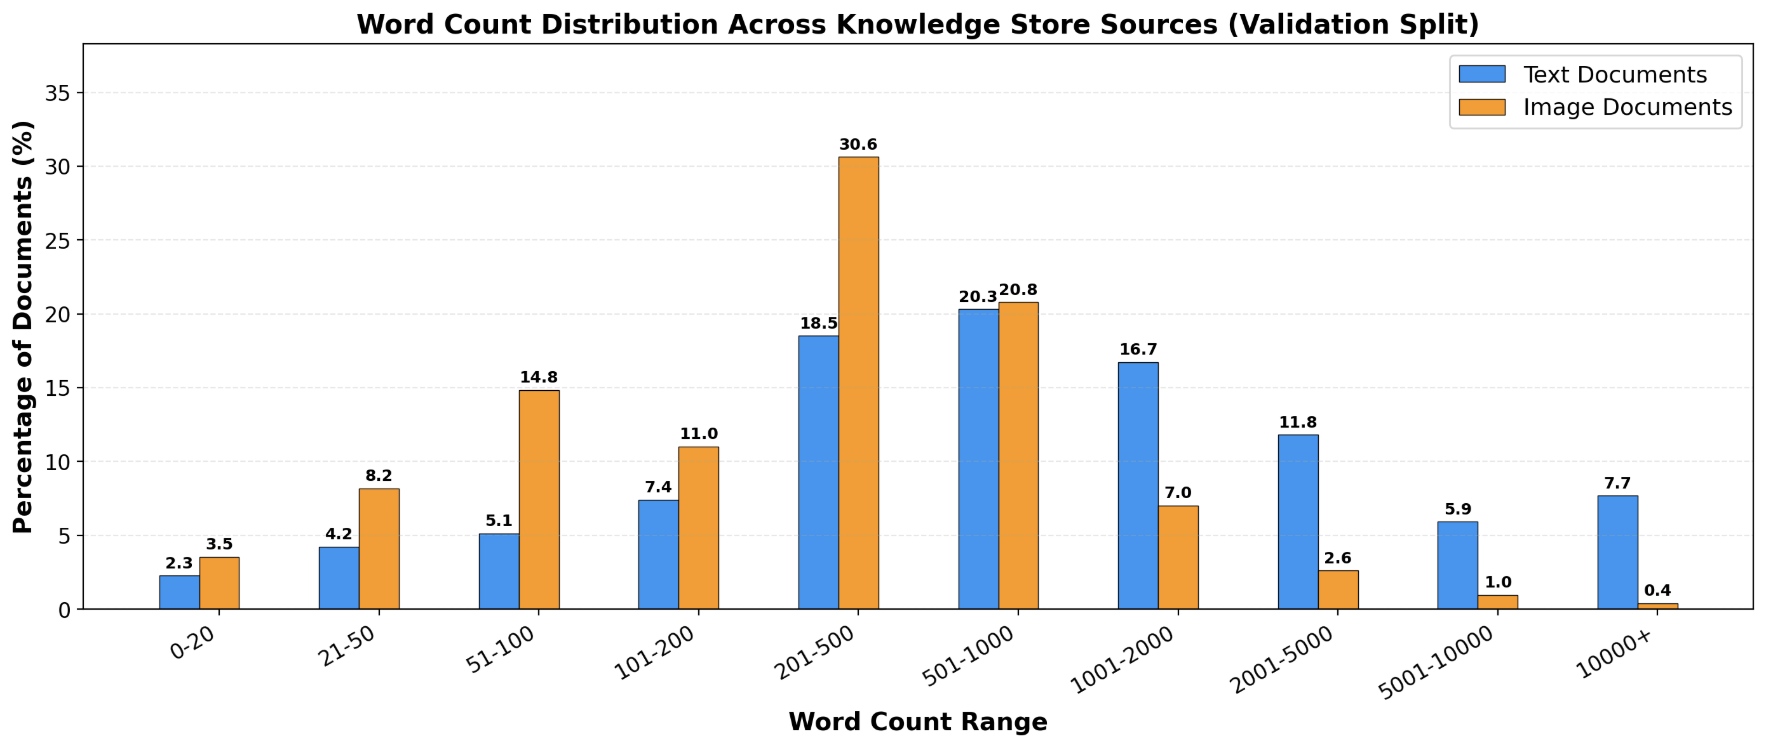
\includegraphics[width=\textwidth]{images/combined_distribution_chart_val.png}
\caption{Word count distribution across knowledge store sources (validation split).}
\label{fig:word_dist_val}
\end{figure}

\begin{figure}[ht]
\centering
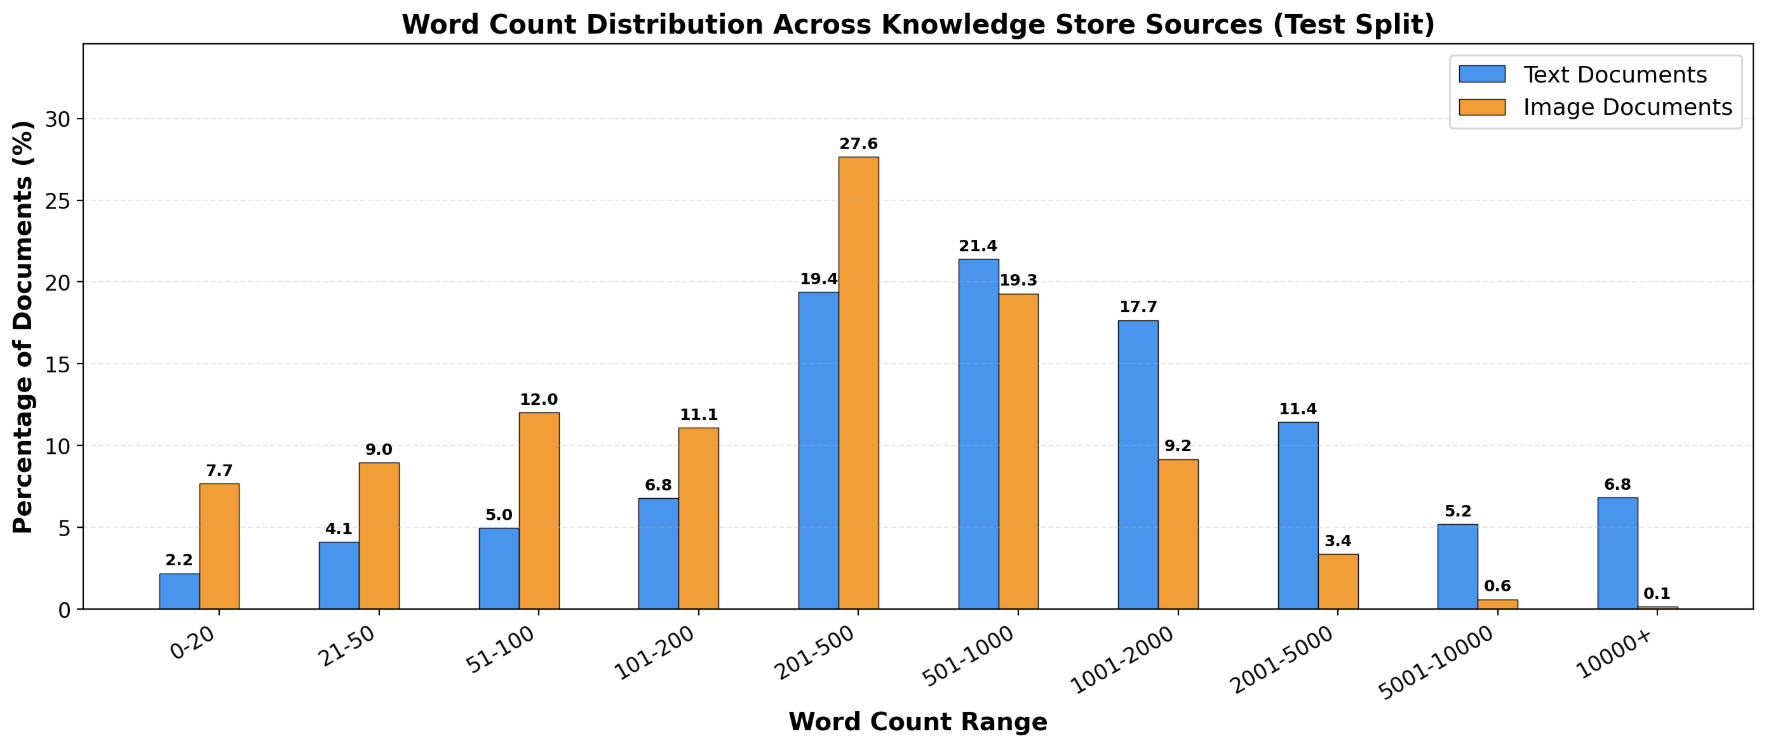
\includegraphics[width=\textwidth]{images/combined_distribution_chart_test.png}
\caption{Word count distribution across knowledge store sources (test split).}
\label{fig:word_dist_test}
\end{figure}

\section{Evaluation Methodology}

The system is evaluated using the official AVerImaTeC shared task evaluation framework, which assesses four core components of the fact-checking pipeline independently: question generation, evidence retrieval, verdict prediction, and justification generation. Additionally, two conditional composite metrics are computed that couple evidence quality with downstream task performance. All VLM-based evaluations use Qwen/Qwen3-VL-8B-Instruct as the evaluation model for validation set.

\subsection{Verdict Prediction Accuracy}

Verdict prediction is evaluated using exact match accuracy. The predicted verdict label is compared case-insensitively against the ground truth label:

\begin{equation}
\text{VerdictAcc}
=
\frac{1}{N}
\sum_{i=1}^{N}
\mathds{1}
\left(
\hat{y}_i = y_i
\right)
\label{eq:verdict_accuracy}
\end{equation}

where $N$ is the total number of evaluated claims, $\hat{y}_i$ denotes the predicted verdict for claim $i$, $y_i$ denotes the corresponding ground-truth verdict, and $\mathds{1}(\cdot)$ is the indicator function, which returns 1 when the predicted verdict matches the ground truth and 0 otherwise. This metric ranges from 0 to 1, with 1 indicating perfect classification accuracy.

\subsection{Question Generation Score}

Question generation quality is measured by computing the recall of reference questions covered by the predicted question set. Two question sets are considered: the predicted questions generated by the system and the reference questions from the ground truth annotations.

The evaluation proceeds in two directions:

\begin{itemize}
    \item \textbf{PRED in REF:} For each predicted question, check whether it is covered by (conveys the same meaning or intent as) any reference question.
    \item \textbf{REF in PRED:} For each reference question, check whether it is covered by any predicted question.
\end{itemize}

Coverage is determined by the VLM evaluator that assesses semantic equivalence rather than exact string matching — two questions are considered equivalent if they convey the same meaning or intent, even if the wording differs.

From these counts, precision, recall, and F1 are computed:

\begin{equation}
    \text{Precision}_Q = \frac{|\text{PRED in REF}|}{|\text{PRED}|}, \quad \text{Recall}_Q = \frac{|\text{REF in PRED}|}{|\text{REF}|}
\end{equation}

\begin{equation}
    F1_Q = \frac{2 \cdot \text{Precision}_Q \cdot \text{Recall}_Q}{\text{Precision}_Q + \text{Recall}_Q}
\end{equation}

The official competition metric uses recall ($\text{Recall}_Q$) as the primary question generation score, measuring what fraction of the ground truth verification questions are covered by the system's generated questions.

\subsection{Evidence Retrieval Score}

Evidence evaluation is the most complex metric, involving both textual and visual evidence comparison. The ground truth evidence is first constructed by converting the reference question-answer pairs into declarative evidence statements (using the same QA-to-evidence conversion described  in \ref{qa_evidence_conversion}). The predicted evidence statements are then compared against these reference statements.

\subsubsection{Textual Evidence Evaluation}

The VLM evaluator compares predicted and reference evidence bidirectionally:

\begin{itemize}
    \item \textbf{PRED in REF:} How many predicted evidence facts are supported by the reference evidence.
    \item \textbf{REF in PRED:} How many reference evidence facts are supported by the predicted evidence.
\end{itemize}

A predicted fact is considered ``supported'' only if the reference evidence contains semantically equivalent information. Importantly, a fact stating ``no answer could be found'' contradicts a reference fact that provides an exact answer, and vice versa — this asymmetry ensures that the system is penalized for failing to find available information.

\subsubsection{Image Evidence Evaluation}

When evidence contains image references (denoted by placeholders like \texttt{[IMG\_1]}, \texttt{[IMG\_2]}), an additional image similarity scoring step is performed. For each matched pair of evidence statements identified in the textual evaluation, the associated images are compared using the VLM-based visual similarity scorer that rates image pair similarity on a 0--10 scale. Images scoring above a threshold of 9 are considered matching.

\subsubsection{Combined Evidence Score}

The final evidence score combines textual and image evaluations into a single recall metric. For each direction (PRED in REF and REF in PRED), the counts from both textual matching and image matching are aggregated:

\begin{equation}
    \text{Precision}_E = \frac{|\text{PRED supported by REF}|}{|\text{PRED}|}, \quad \text{Recall}_E = \frac{|\text{REF supported by PRED}|}{|\text{REF}|}
\end{equation}

\begin{equation}
    F1_E = \frac{2 \cdot \text{Precision}_E \cdot \text{Recall}_E}{\text{Precision}_E + \text{Recall}_E}
\end{equation}

The official competition uses recall ($\text{Recall}_E$) as the primary evidence retrieval score.

\subsection{Justification Score}

Justification evaluation decomposes both the predicted and reference justifications into atomic facts and then measures how well the predicted justification covers the reference facts.

The evaluation process:

\begin{enumerate}
    \item \textbf{Decomposition:} The VLM evaluator decomposes the predicted justification into atomic facts (PRED\_FACT) and the reference justification into atomic facts (REF\_FACT). Each atomic fact is a single, self-contained sentence expressing one piece of information.
    \item \textbf{Bidirectional coverage:} Each predicted fact is checked for coverage by the reference facts, and each reference fact is checked for coverage by the predicted facts.
    \item \textbf{Recall computation:} The justification recall measures what fraction of the reference atomic facts are covered by the predicted justification.
\end{enumerate}

\begin{equation}
    \text{Justification\_Recall} = \frac{|\text{REF\_FACT covered by PRED\_FACT}|}{|\text{REF\_FACT}|}
\end{equation}

This recall-based metric rewards justifications that capture the key reasoning elements present in the ground truth explanation, without penalizing the inclusion of additional valid reasoning steps.

\subsection{Conditional Composite Metrics}

The official AVerImaTeC evaluation introduces two conditional composite metrics that gate downstream scores on evidence quality. These metrics reflect the intuition that a correct verdict or justification is only meaningful if it is grounded in sufficient evidence.

\subsubsection{Evidence-Conditioned Verdict Score}

The evidence-conditioned verdict score counts a sample's verdict as correct only when the evidence retrieval score exceeds a threshold $\lambda = 0.3$:

\begin{equation}
\text{EVScore}
=
\frac{1}{N}
\sum_{i=1}^{N}
\mathds{1}
\left(
R_{E,i} > \lambda
\right)
\cdot
\mathds{1}
\left(
\hat{y}_i = y_i
\right)
\label{eq:evidence_verdict_score}
\end{equation}

where $N$ is the total number of evaluated claims, $R_{E,i}$ denotes the evidence recall score for claim $i$, $\lambda$ is the evidence quality threshold, $\hat{y}_i$ denotes the predicted verdict, $y_i$ denotes the ground-truth verdict, and $\mathds{1}(\cdot)$ is the indicator function. The metric assigns a score of 1 only when the predicted verdict is correct and the retrieved evidence exceeds the specified recall threshold. The final score is obtained by averaging over all evaluated claims.

This metric penalizes systems that achieve correct verdicts through lucky guessing rather than through retrieval of relevant evidence. A system that predicts the correct verdict but fails to retrieve supporting evidence (scoring below 0.3 on evidence recall) receives no credit for that sample.

\subsubsection{Evidence-Conditioned Justification Score}

Similarly, the evidence-conditioned justification score gates the justification recall on evidence quality:

\begin{equation}
\text{EJScore}
=
\frac{1}{N}
\sum_{i=1}^{N}
\mathds{1}
\left(
R_{E,i} > \lambda
\right)
\cdot
J_i
\label{eq:evidence_justification_score}
\end{equation}

where $J_i$ denotes the justification quality score for claim $i$.

This ensures that justification quality is only measured for samples where the system has demonstrated the ability to retrieve relevant evidence, filtering out justifications that may be well-written but not grounded in retrieved facts.

\subsection{Summary of Evaluation Metrics}

Table~\ref{tab:eval_metrics} summarizes the evaluation metrics used in the official AVerImaTeC shared task.

\begin{table}[htbp]
\centering
\caption{Summary of evaluation metrics used in the AVerImaTeC shared task.}
\label{tab:eval_metrics}
\begin{tabular}{lll}
\hline
\textbf{Metric} & \textbf{Type} & \textbf{Description} \\
\hline
Question Generation & Recall & Reference questions covered by predictions \\
Evidence Retrieval & Recall & Reference evidence supported by predictions \\
Verdict Prediction & Accuracy & Exact match of predicted vs.\ ground truth label \\
Justification & Recall & Reference atomic facts covered by prediction \\
Evidence-Verdict & Conditional & Verdict accuracy gated on evidence $> 0.3$ \\
Evidence-Justification & Conditional & Justification recall gated on evidence $> 0.3$ \\
\hline
\end{tabular}
\end{table}

All VLM-based evaluations (question generation, evidence retrieval, and justification) use an evaluator model that scores semantic equivalence rather than lexical overlap, ensuring that systems are not penalized for valid paraphrases or alternative phrasings that convey the same factual content.

\subsection{Evaluation Protocol}

We used the validation and test datasets for evaluation following a two-stage protocol. First, the validation set (152 claims) was used for iterative development and ablation studies. All six metrics were monitored across experiments to ensure that pipeline modifications led to consistent improvements and did not cause regressions. Second, the test set (352 claims) was used for final evaluation on completely unseen data, with scores computed by the official competition server. This two-stage approach ensures that results on the test set reflect genuine generalization rather than overfitting to a particular data split.

\section{Experimental Results}
This section presents the experimental results. The results are organized according to the research questions (RQs) defined in the introduction. For each RQ, we present the relevant results and provide an analysis of the findings.

Table~\ref{tab:hyperparams} lists the key hyperparameters used in the pipeline. These values were selected through empirical tuning on the validation set. Lower temperatures (0.2) were used for verdict and justification generation to maximize determinism and factual consistency, while a moderate temperature (0.5) was used for QA generation to encourage diverse question. The MMR diversity parameter $\lambda = 0.5$ provides an equal balance between relevance and diversity in the final evidence set. The RRF constant $K = 60$ follows the standard recommendation from the original RRF formulation~\cite{Rackauckas2024Jan}, which controls the diminishing influence of lower-ranked documents. Top-$K = 50$ was chosen to provide sufficient retrieval recall while keeping the computational cost of downstream reranking manageable.

\begin{table}[ht]
\centering
\caption{Pipeline hyperparameters.}
\label{tab:hyperparams}
\begin{tabular}{lr}
\hline
\textbf{Parameter} & \textbf{Value} \\
\hline

VLM temperature (QA generation)             & 0.5 \\
VLM temperature (verdict generation)        & 0.2 \\
VLM temperature (justification generation)  & 0.2 \\
MMR diversity $\lambda$                      & 0.5 \\
RRF $K$ parameter                            & 60  \\
Top-$K$ (SPLADE, BGE, LongCLIP)             & 50  \\
\hline
\end{tabular}
\end{table}

\subsection{RQ1: How do the individual retrieval modalities (SPLADE, BGE, LongCLIP) and post-retrieval stages (cross-encoder reranking, MMR diversification) contribute to downstream fact-checking performance?}

To answer \textbf{RQ1}, we perform an incremental ablation study on the retrieval pipeline using the validation set with ground truth questions. This isolates the effect of each retrieval modality and post-retrieval stage from the question generation component. Table~\ref{tab:retrieval_ablation} presents the results.

\begin{table}[ht]
\centering
\caption{Retrieval ablation results on the validation set with ground truth questions.}
\label{tab:retrieval_ablation}
\resizebox{\textwidth}{!}{
\begin{tabular}{lccccc}
\hline
\textbf{Retrieval Type} & \textbf{\makecell{Evidence\\Score}} & \textbf{\makecell{Verdict\\Score}} & \textbf{\makecell{Justification\\Score}} & \textbf{\makecell{Evidence\\Verdict}} & \textbf{\makecell{Evidence\\Justification}}\\
\hline
SPLADE                    & 0.34 & 0.63 & 0.30 & 0.31 & 0.22\\
BGE                       & 0.24 & 0.60 & 0.27 & 0.19 & 0.14\\
SPLADE+BGE                & 0.34 & 0.63 & 0.33 & 0.31 & 0.22 \\
SPLADE+BGE+CLIP           & 0.31 & 0.645 & 0.363 & 0.29 & 0.21 \\
SPLADE+BGE+LongCLIP   & 0.40 & 0.66 & 0.40 & 0.40 & 0.32 \\
With Cross Encoder        & 0.42 & 0.664 & 0.41 & 0.40 & 0.32 \\
\textbf{With MMR}                  & \textbf{0.45} & \textbf{0.71} & \textbf{0.44} & \textbf{0.46} & \textbf{0.35} \\
\hline
\end{tabular}
}
\end{table}

Several observations emerge from this ablation. First, SPLADE alone outperforms BGE on evidence score (0.34 vs.\ 0.24), confirming the importance of learned sparse lexical matching for fact-checking where exact entity and keyword overlap is critical. The combination of SPLADE+BGE does not improve evidence score over SPLADE alone, but yields a modest gain in justification score (0.33 vs.\ 0.30), suggesting that dense retrieval contributes complementary semantic information useful for generating justifications.

Second, adding standard CLIP to the hybrid retriever actually decreases evidence score from 0.34 to 0.31. This is attributable to CLIP's 77-token text limit, which causes it to focus on superficial image-text alignment rather than the longer contextual evidence needed for fact verification. Replacing CLIP with LongCLIP produces a substantial improvement across all metrics: evidence score increases from 0.31 to 0.40 (+29\%), and evidence-conditioned verdict score increases from 0.29 to 0.40. This validates the hypothesis that long-context visual grounding is essential for multimodal fact-checking.

Third, the post-retrieval stages provide further gains. Cross-encoder reranking improves evidence score from 0.40 to 0.42 by refining the ranking quality through full query-document interaction. The most significant single-stage improvement comes from MMR diversification, which raises the evidence score from 0.42 to 0.45 and the verdict score from 0.66 to 0.71. This demonstrates that reducing redundancy in the retrieved evidence set allows the VLM to reason over a more comprehensive set of facts, directly improving downstream verdict accuracy. Figure~\ref{fig:confusion_matrix_mmr} visualizes this effect through confusion matrices, showing that MMR improves verdict accuracy from 66.4\% to 71\%, primarily by correctly classifying more \textit{Refuted} claims.

\begin{figure}[ht]
\centering
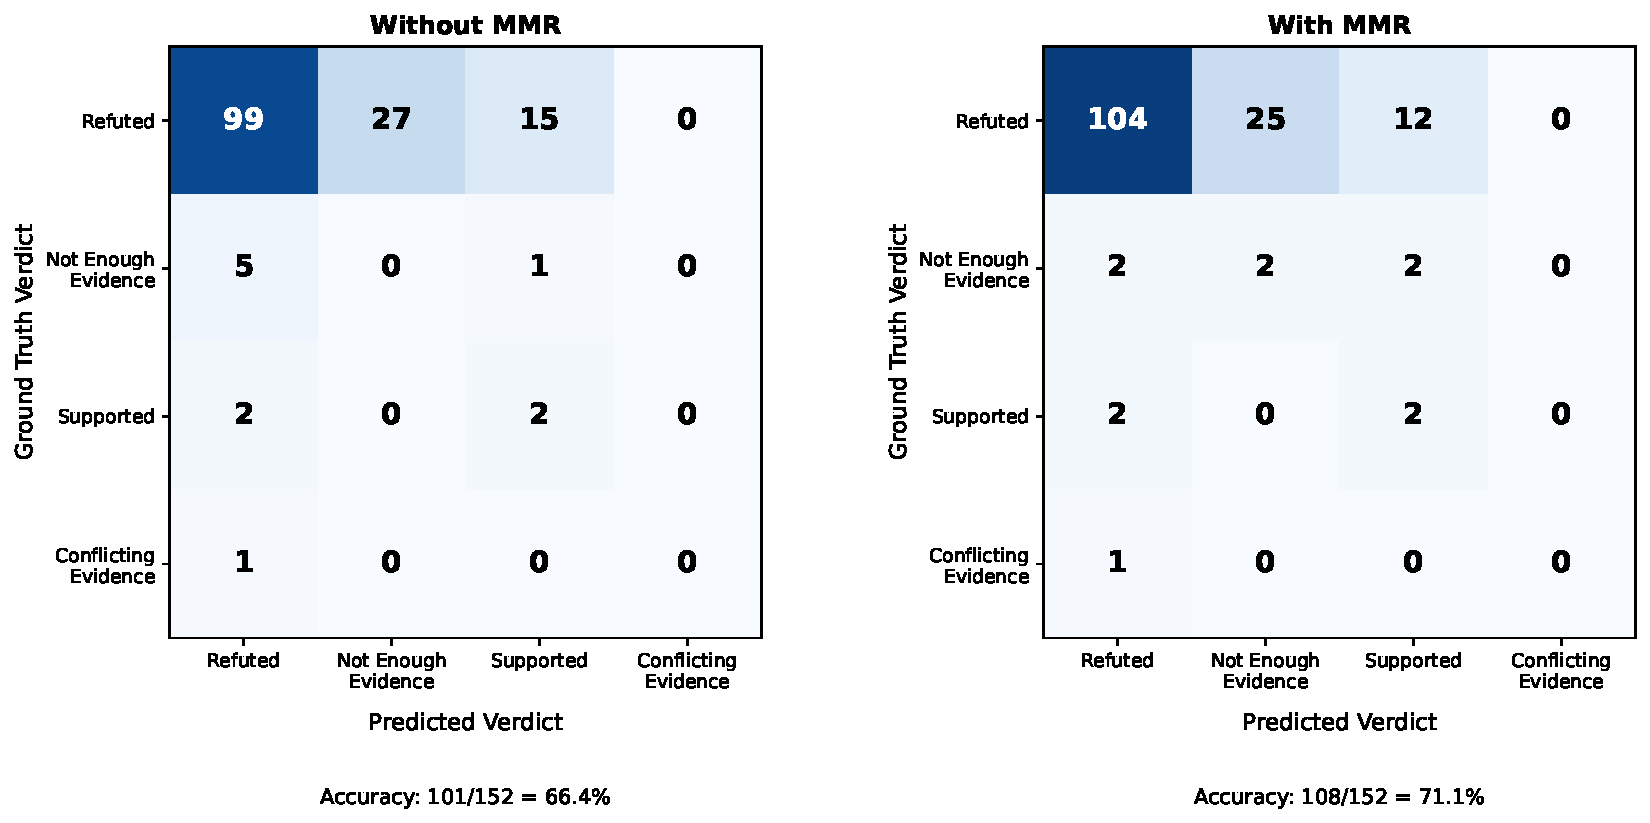
\includegraphics[width=\textwidth]{images/confusion_matrix_mmr.pdf}
\caption{Confusion matrices for verdict prediction on the validation set comparing the effect of MMR diversification. Left: without MMR. Right: with MMR.}
\label{fig:confusion_matrix_mmr}
\end{figure}

The cumulative effect of the full pipeline (SPLADE+BGE+LongCLIP+Cross-Encoder+MMR) yields a 32\% relative improvement in evidence score over the SPLADE-only baseline (0.45 vs.\ 0.34) and a 46\% improvement in justification score (0.44 vs.\ 0.30).

Table~\ref{tab:retrieval_ablation_test} further confirms these findings on the test set, where replacing standard CLIP with LongCLIP improves evidence score by 29\% (0.173 to 0.224) and verdict score by 30\% (0.176 to 0.23).

\begin{table}[ht]
\centering
\caption{Effect of retrieval type in iterative QA generation pipeline on the test set.}
\label{tab:retrieval_ablation_test}
\begin{tabular}{lcccc}
\hline
\textbf{Retrieval} & \textbf{\makecell{Question\\ Score}} & \textbf{\makecell{Evidence\\ Score}} & \textbf{\makecell{Verdict\\Score}} & \textbf{\makecell{Justification\\ Score}}  \\
\hline
SPLADE+BGE+CLIP  & 0.486 & 0.173 & 0.176 & 0.154  \\
\textbf{SPLADE+BGE+LongCLIP} & \textbf{0.495} & \textbf{0.224} & \textbf{0.23} & \textbf{0.17}\\
\hline
\end{tabular}
\end{table}

\subsection{RQ2: How does iterative question-answer generation compare to a claim based retrieval for QA generation in terms of evidence quality and verdict accuracy?}

To answer \textbf{RQ2}, we compare two QA generation strategies: (1)~iterative question generation, where questions are generated iteratively followed by evidence retrieval and answer generation ; and (2)claim based retrieval for QA generation (single pass), where all questions and answers are generated in a single VLM call after retrieving evidence. Both configurations use the full retrieval pipeline (SPLADE+BGE+LongCLIP+Cross-Encoder+MMR).

Table~\ref{tab:icl_ablation} shows the iterative approach on the validation set, while Table~\ref{tab:one_go_val} shows the single pass approach.

\begin{table}[ht]
\centering
\caption{Iterative QA generation pipeline performance on the validation set.}
\label{tab:icl_ablation}
\resizebox{\textwidth}{!}{
\begin{tabular}{lcccccc}
\hline
\textbf{\makecell{In-context \\Learning}} & \textbf{\makecell{Question\\ Score}} & \textbf{\makecell{Evidence\\ Score}} & \textbf{\makecell{Verdict\\Score}} & \textbf{\makecell{Justification\\ Score}} & \textbf{\makecell{Evidence\\ Verdict}} & \textbf{\makecell{Evidence\\Justification}} \\
\hline
No  & 0.18 & 0.16 & 0.704 & 0.336 & 0.236 & 0.157 \\
\textbf{Yes} & \textbf{0.34} & \textbf{0.214} & \textbf{0.724} & \textbf{0.363}  & \textbf{0.26} & \textbf{0.19} \\
\hline
\end{tabular}
}
\end{table}

\begin{table}[ht]
\centering
\caption{Single pass QA generation pipeline performance on the validation set.}
\label{tab:one_go_val}
\resizebox{\textwidth}{!}{
\begin{tabular}{lcccccc}
\hline
\textbf{\makecell{In-context \\Learning}} & \textbf{\makecell{Question\\ Score}} & \textbf{\makecell{Evidence\\ Score}} & \textbf{\makecell{Verdict\\Score}} & \textbf{\makecell{Justification\\ Score}} & \textbf{\makecell{Evidence\\ Verdict}} & \textbf{\makecell{Evidence\\Justification}} \\
\hline
\textbf{No}  & \textbf{0.35} & \textbf{0.237} & \textbf{0.81} & \textbf{0.42} & \textbf{0.29} & \textbf{0.22} \\
Yes & 0.4 & 0.23 & 0.77 & 0.37  & 0.28 & 0.22 \\
\hline
\end{tabular}
}
\end{table}


Comparing the best configuration of each strategy (iterative with ICL vs.\ single pass without ICL), the single-pass approach substantially outperforms iterative generation across all metrics: question score (0.35 vs.\ 0.34), evidence score (0.237 vs.\ 0.214), verdict score (0.81 vs.\ 0.72), and justification score (0.42 vs.\ 0.363).

This result suggests that generating all questions and answers in a single coherent pass after evidence retrieval allows the VLM to maintain better contextual consistency and produce more holistic verification reasoning. The iterative approach, while theoretically allowing refinement across iterations, appears to suffer from error propagation—poor early questions lead to irrelevant evidence retrieval, which in turn degrades subsequent question generation.

On the test set (Table~\ref{tab:one_go_test}), the single approach with ICL achieves a question score of 0.622, evidence score of 0.312, verdict score of 0.327, and justification score of 0.297—representing our best test set submission. Notably, ICL improves all metrics on the test set despite hurting validation performance, suggesting that the few-shot examples provide better generalization to unseen claims even when they constrain validation-set verdict accuracy.

\begin{table}[ht]
\centering
\caption{Single pass QA generation pipeline performance on the test set.}
\label{tab:one_go_test}
\begin{tabular}{lcccc}
\hline
\textbf{\makecell{In-context \\Learning}} & \textbf{\makecell{Question\\ Score}} & \textbf{\makecell{Evidence\\ Score}} & \textbf{\makecell{Verdict\\Score}} & \textbf{\makecell{Justification\\ Score}} \\
\hline
No  & 0.634 & 0.277 & 0.289 & 0.265\\
\textbf{Yes} & \textbf{0.622} & \textbf{0.312} & \textbf{0.327} & \textbf{0.297}\\
\hline
\end{tabular}
\end{table}


\subsection{RQ3: What is the effect of in-context learning on question generation quality and overall pipeline performance?}

To answer \textbf{RQ3}, we examine the impact of in-context learning (ICL) on both generation strategies. In the ICL setting, all-MiniLM-L6-v2 Bert model is used to retrieve similar QA-pair examples from the training set, which are included in the VLM prompt as few-shot demonstrations.

For \textit{iterative QA generation} (Table~\ref{tab:icl_ablation}), ICL provides a clear benefit: question score nearly doubles from 0.18 to 0.34, and all downstream metrics improve correspondingly. ICL helps the VLM understand the expected question format and granularity, producing more targeted verification questions.

For \textit{Single pass QA generation} (Table~\ref{tab:one_go_val}), the effect of ICL is mixed on the validation set. While question score improves from 0.35 to 0.4, the verdict score drops from 0.81 to 0.77 and justification score from 0.42 to 0.37. This suggests that in the single pass setting, few-shot examples may constrain the VLM's reasoning, causing it to mimic the structure of training examples rather than adapting to the specific claim. The retrieved ICL examples may introduce noise when the test claim differs substantially from the training distribution.

On the test set (Table~\ref{tab:one_go_test}), the pattern reverses: ICL improves all metrics, with evidence score rising from 0.277 to 0.312 (+12\%), verdict score from 0.289 to 0.327 (+13\%), and justification score from 0.265 to 0.297 (+12\%). This reversal suggests that while ICL constrains the VLM on the heavily imbalanced validation set (where unconstrained reasoning exploits majority-class bias), it provides valuable structural guidance on the more diverse test distribution, helping the model generate better-formed questions and more grounded answers.

\textbf{Takeaway:} ICL is consistently beneficial for iterative generation. For single-pass generation, ICL reduces validation verdict accuracy but improves generalization to unseen test data—indicating that the validation verdict gains without ICL may be partially attributable to majority-class bias rather than genuine reasoning quality.

To further illustrate the impact of ICL on verdict prediction, Figures~\ref{fig:confusion_matrix_iterative} and~\ref{fig:confusion_matrix_retrieval_first} present confusion matrices for both generation strategies. In the iterative setting (Figure~\ref{fig:confusion_matrix_iterative}), ICL improves accuracy from 70.4\% to 72.4\%, primarily by reducing misclassifications of \textit{Refuted} claims as \textit{Not Enough Evidence}. In the single pass setting (Figure~\ref{fig:confusion_matrix_retrieval_first}), removing ICL yields 81\% accuracy compared to 77\% with ICL, confirming that few-shot examples constrain the VLM's reasoning on the validation set.

\begin{figure}[ht]
\centering
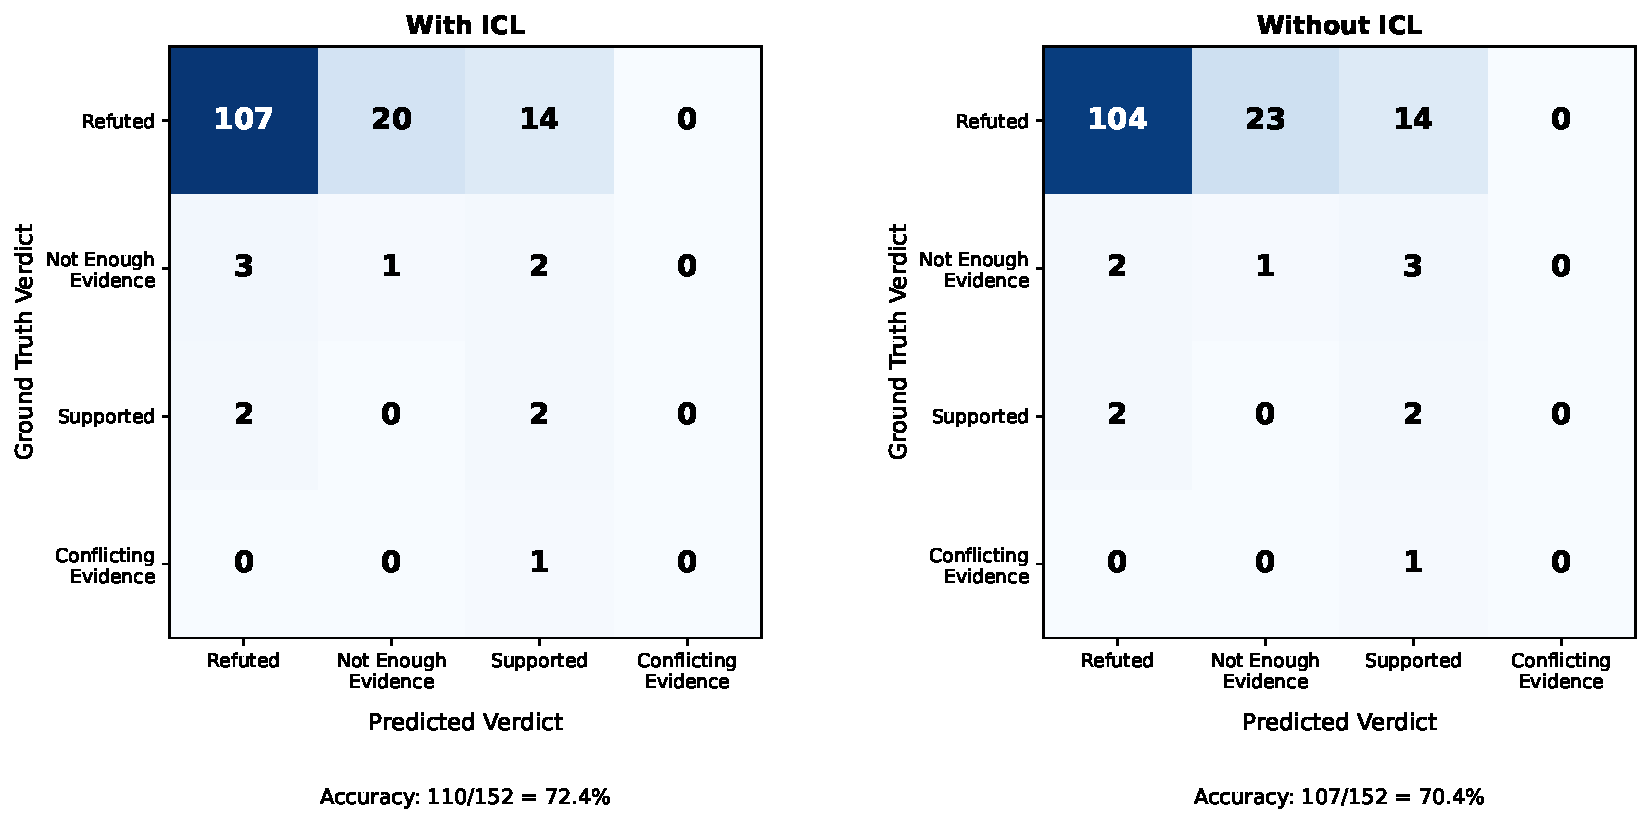
\includegraphics[width=\textwidth]{images/confusion_matrix_iterative.pdf}
\caption{Confusion matrices for verdict prediction using the iterative QA generation strategy on the validation set. Left: with in-context learning. Right: without in-context learning.}
\label{fig:confusion_matrix_iterative}
\end{figure}

\begin{figure}[ht]
\centering
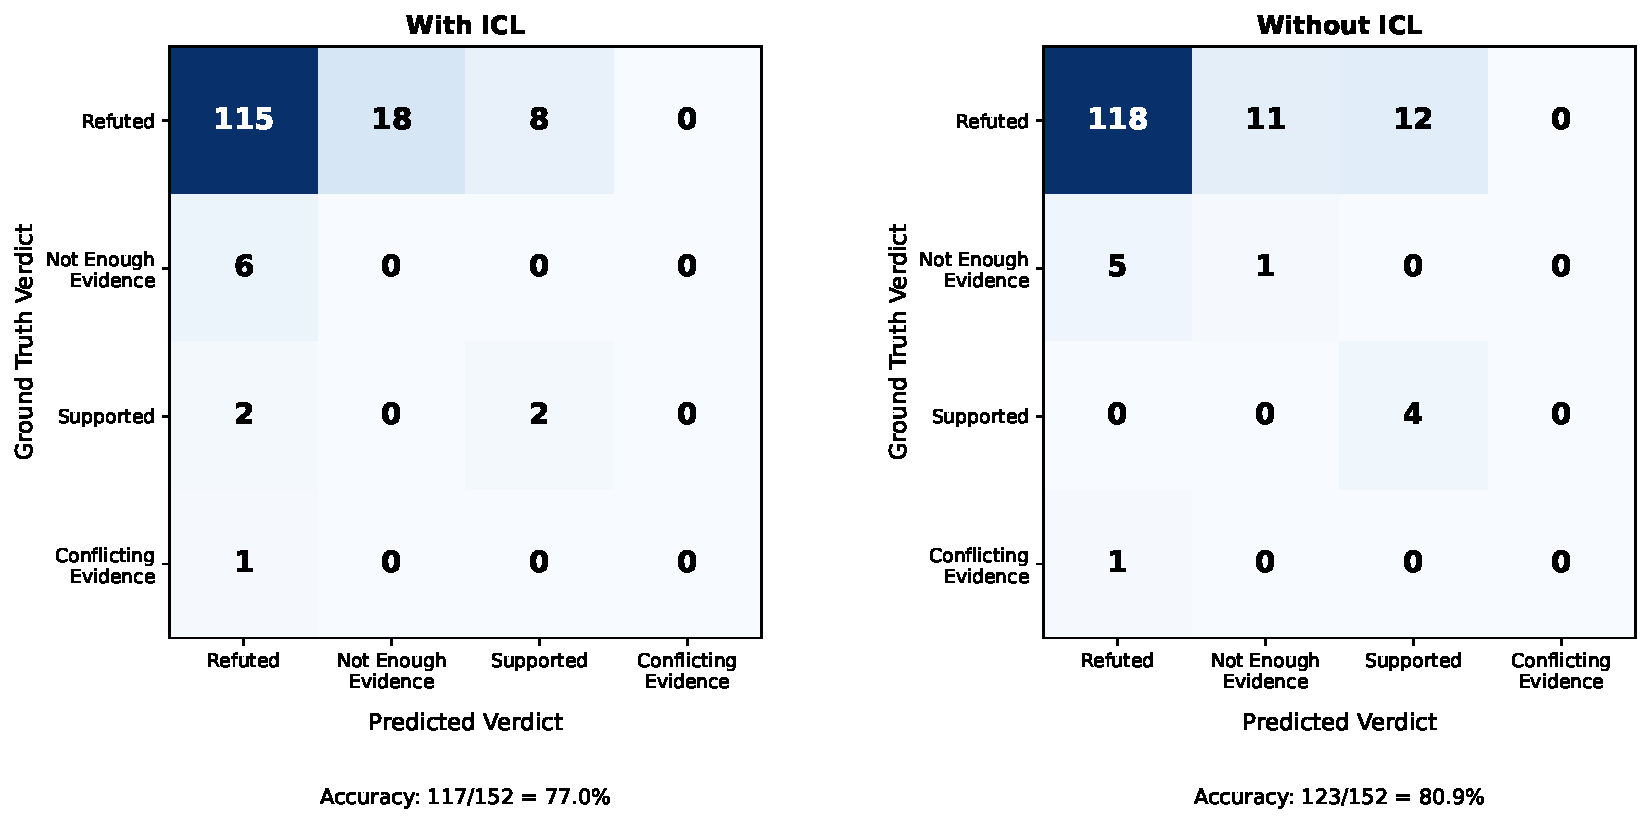
\includegraphics[width=\textwidth]{images/confusion_matrix_retrieval_first.pdf}
\caption{Confusion matrices for verdict prediction using the single-pass QA generation strategy on the validation set. Left: with in-context learning. Right: without in-context learning.}
\label{fig:confusion_matrix_retrieval_first}
\end{figure}

\subsection{RQ4: How does the proposed pipeline compare to state-of-the-art systems on the AVerImaTeC shared task?}

To answer \textbf{RQ4}, we compare our best pipeline configuration against the top-performing teams in the AVerImaTeC shared task. Tables~\ref{tab:team_comparison_val} and~\ref{tab:team_comparison_test} present results on the validation and test sets respectively.

\begin{table}[ht]
\centering
\caption{Comparison with other teams on the validation set.}
\label{tab:team_comparison_val}
\begin{tabular}{lcccc}
\hline
\textbf{Team} & \textbf{\makecell{Question\\Score}} & \textbf{\makecell{Evidence\\Score}} & \textbf{\makecell{Verdict\\Score}} & \textbf{\makecell{Justification\\Score}} \\
\hline
VILLAIN  & 0.9228 & 0.5832 & 0.6447 & 0.5427 \\
ADA-AGGR  & 0.3539 & 0.3864 & 0.4539 & 0.3727 \\
AIC CTU    & 0.8223 & 0.3466 & 0.375 & 0.3035 \\
\textbf{Single-pass No-Icl (Ours)}     & \textbf{0.35} & \textbf{0.237} & \textbf{0.81} & \textbf{0.42} \\
Xxp        & 0.3729 & 0.2227  & 0.2303 & 0.175 \\
fv         & 0.4299 & 0.1614 & 0.1645 & 0.1179 \\
Baseline & 0.4882 & 0.1335 & 0.0658 & 0.0576 \\

\hline
\end{tabular}
\end{table}

The final validation score used to compare to other frameworks in validation set is a single pass question-answer generation with no in-context learning.

The final system configuration, consisting of hybrid multimodal dual-branch  retrieval, single-pass question-answer generation, and in-context learning, is referred to as HyMFact and is used for all official test-set comparisons.
\begin{table}[ht]
\centering
\caption{Comparison with other teams on the test set.}
\label{tab:team_comparison_test}
\begin{tabular}{lcccc}
\hline
\textbf{Team} & \textbf{\makecell{Question\\Score}} & \textbf{\makecell{Evidence\\Score}} & \textbf{\makecell{Verdict\\Score}} & \textbf{\makecell{Justification\\Score}} \\
\hline
VILLAIN  & 0.8897 & 0.5358 & 0.5455 & 0.5557 \\
ADA-AGGR   & 0.3701 & 0.4629 & 0.5369 & 0.4331 \\
AIC-CTU   & 0.8065 & 0.3251 & 0.3466 & 0.3043 \\
\textbf{HyMFact (Ours)}     & \textbf{0.622} & \textbf{0.312} & \textbf{0.327} & \textbf{0.297} \\
Xxp         & 0.3902 & 0.2703 & 0.2557 & 0.198 \\
REVEAL      & 0.6317 & 0.2771 & 0.2358 & 0.1348 \\
fv          & 0.2885 & 0.1626 & 0.1591 & 0.1306 \\
Baseline & 0.2885 & 0.1707 & 0.1591 & 0.1306 \\
\hline
\end{tabular}
\end{table}

On the validation set, our system achieves the highest verdict score (0.81) among all teams, substantially outperforming the first-place HUMANE system (0.6447) by over 16 percentage points. This demonstrates that our hybrid retrieval pipeline combined with single-pass VLM reasoning produces highly accurate verdict predictions when evaluated locally. Our justification score (0.42) also exceeds all systems except VILLAIN.

However, our question score (0.35) and evidence score (0.237) are lower than most competing systems. This gap is primarily attributable to two factors: (1)~our use of a smaller VLM (Qwen3-VL-8B) compared to the proprietary MLLMs used by other teams (GPT-5.1, Gemini-2.5-Pro), which limits question generation diversity; and (2)~we generate fewer questions (5) than other teams.

On the test set, the performance gap between validation and test is notable: our best verdict score drops from 0.81 (validation, without ICL) to 0.327 (test, with ICL). This discrepancy suggests that the high validation verdict accuracy is partially inflated by the extreme class imbalance (90\% Refuted), and the test set likely contains a more balanced label distribution. Notably, our best test configuration uses ICL, which achieves lower validation scores but generalizes better. Despite the val-to-test gap, our system outperforms the baseline across all metrics and achieves competitive evidence and justification scores relative to the proprietary MLLM-based systems, while using significantly fewer computational resources (a single 8B-parameter open-source VLM vs.\ multiple calls to commercial MLLMs).

\section{Discussion}
\label{sec:discussion}

This section synthesizes the findings across all research questions and discusses their broader implications for multimodal fact-checking pipeline design.

\subsection{Retrieval as the Performance Bottleneck}

Across all experimental configurations, evidence retrieval score consistently remains the weakest component of the pipeline. Even our best configuration achieves only 0.312 evidence score on the test set, compared to 0.622 for question generation and 0.327 for verdict prediction. This pattern is consistent across competing systems: even the top-ranked VILLAIN system achieves only 0.5358 evidence score despite scoring 0.8897 on question generation.

This finding suggests that retrieval—not reasoning—is the primary bottleneck in current multimodal fact-checking systems. The implication for future work is clear: improvements in retrieval quality are likely to yield larger downstream gains than improvements in the VLM reasoning component. Our ablation study (RQ1) confirms this, showing that each retrieval enhancement (LongCLIP, cross-encoder, MMR) propagates improvements to all downstream metrics.

\subsection{Open-Source VLM vs.\ Proprietary MLLM Trade-off}

A key design decision in our pipeline is the use of Qwen3-VL-8B-Instruct, an open-source 8B-parameter VLM, while competing systems rely on proprietary MLLMs such as GPT-5.1, Gemini-2.5-Pro and Gemini 3 Pro. This choice involves a clear trade-off:

\begin{itemize}
    \item \textbf{Advantages:} Full reproducibility, no API costs, ability to run locally on a single A100 GPU, no rate limiting, and complete control over inference parameters.
    \item \textbf{Disadvantages:} Lower question generation diversity (0.622 vs.\ 0.890 for VILLAIN), reduced capacity for complex multi-hop reasoning, and smaller context window limiting the amount of evidence that can be processed simultaneously.
\end{itemize}

Despite these limitations, our system achieves competitive verdict and justification performance, demonstrating that a well-designed retrieval pipeline can partially compensate for a smaller reasoning model. The evidence score gap (0.312 vs.\ 0.536) suggests that retrieval quality, rather than model size alone, is a significant differentiator.

\subsection{The Role of Evidence Diversity}

One of the clearest findings from RQ1 is the outsized impact of MMR diversification on downstream performance. MMR improved all scores in the validation set. This suggests that providing the VLM with diverse, non-redundant evidence is more important than providing the highest-scoring evidence alone.

This finding has practical implications: in retrieval-augmented fact-checking, evidence selection strategies that prioritize coverage over raw relevance are more effective. The VLM benefits from seeing multiple perspectives and complementary pieces of information rather than multiple similar passages that all express the same fact.

\subsection{Validation Metrics as Unreliable Predictors}

The val-to-test gap (0.81 to 0.327 verdict score) reveals a cautionary lesson about evaluation on small, imbalanced datasets. The 152-claim validation set with over 90\% Refuted labels creates conditions where a system can achieve high accuracy through implicit bias rather than genuine reasoning. The test set, with its larger size and potentially more balanced distribution, provides a more realistic assessment of system capability.

We attribute the generalization gap to three factors: (1)~\textbf{label distribution shift}---if the test set has a more balanced distribution, our model's implicit bias toward predicting Refuted becomes counterproductive; (2)~\textbf{claim complexity}---the test set is substantially larger (352 vs.\ 152 claims) and may contain more diverse claim types not well-represented in validation; and (3)~\textbf{knowledge store scale}---the test knowledge store contains 5$\times$ more documents (503K vs.\ 99K text documents), increasing the search space and potentially introducing more distracting content that degrades retrieval precision.

This finding also explains the ICL paradox observed in RQ3: ICL reduces validation verdict score (from 0.81 to 0.77) but improves test performance (from 0.289 to 0.327). Without ICL, the VLM develops an unconstrained bias toward the majority class that inflates validation accuracy but fails to generalize. ICL introduces structural constraints that reduce this bias, resulting in lower but more honest validation scores and better generalization.

\subsection{Limitations}

Several limitations should be acknowledged:

\begin{itemize}
    \item \textbf{Dataset scale:} The AVerImaTeC dataset contains only 1,297 claims total, with 152 for validation. Results on such a small dataset may not be statistically robust, and small performance differences may not be significant.
    \item \textbf{Class imbalance:} The extreme imbalance (over 90\% Refuted) in the known splits makes it difficult to assess performance on minority classes. The system's ability to correctly identify Supported or Conflicting Evidence claims remains largely untested.
    \item \textbf{Single VLM backbone:} All results are obtained with Qwen3-VL-8B-Instruct. The findings regarding ICL effects and generation strategies may not transfer to other model families or sizes.
    \item \textbf{Fixed knowledge store:} The evaluation assumes a pre-constructed knowledge store. In real-world deployment, the system would need to handle dynamic evidence retrieval from the open web, which introduces additional challenges.
\end{itemize}


\section{Qualitative Examples}
\label{sec:qualitative}

To complement the quantitative evaluation, we present representative examples that illustrate the system's behavior in both success and failure cases.

\subsection{Success Case: Multimodal Retrieval Advantage}

To illustrate the advantage of multimodal retrieval, we examine Sample~82 from the validation set. The claim states: \textit{``Woman seen with Dawood in the photo from 1987 is Supriya Shrinate.''} The claim image (Figure~\ref{fig:success_case}) shows a woman sitting next to a man, and the ground truth identifies her as journalist Sheela Bhatt interviewing Dawood Ibrahim in Dubai in 1987.

\begin{figure}[ht]
\centering
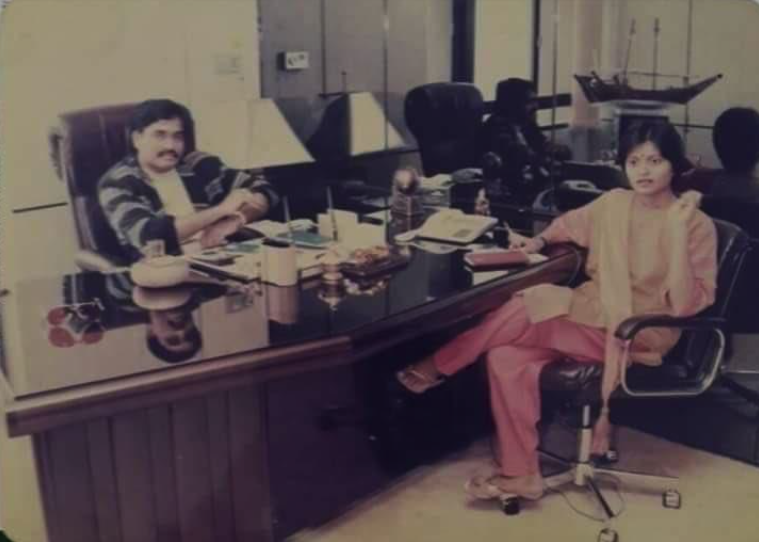
\includegraphics[width=0.6\textwidth]{images/claim82.png}
\caption{Success case: claim image where LongCLIP retrieval identified key visual evidence that text-only retrieval missed.}
\label{fig:success_case}
\end{figure}

\begin{table}[ht]
\centering
\caption{Comparison of text-only vs.\ multimodal retrieval for Sample~82.}
\label{tab:longclip_success_case}
\begin{tabular}{p{0.22\textwidth} p{0.34\textwidth} p{0.34\textwidth}}
\toprule
\textbf{Component} & \textbf{SPLADE+BGE (text-only)} & \textbf{With LongCLIP (multimodal)} \\
\midrule
Answer & No answer was found & Sheela Bhatt interviewing Dawood Ibrahim in 1987 \textcolor{green}{(\ding{51})} \\
\midrule
Evidence Score & 0.0 & 0.5 \\
Verdict & Not Enough Evidence \textcolor{red}{(\ding{55})} & Refuted \textcolor{green}{(\ding{51})} \\
GT Verdict & Refuted & Refuted \\
\bottomrule
\end{tabular}
\end{table}

Using only text-based retrieval (SPLADE+BGE), the system could not find evidence identifying the woman in the photograph, returning ``no answer found''. This is because the relevant evidence is associated with a web page found through reverse image search---it is indexed under the image modality, not the text documents. Without visual retrieval, no amount of keyword or semantic text matching can surface this evidence.

By incorporating LongCLIP, the claim image was matched against embeddings generated from image-related textual documents, enabling retrieval of evidence that correctly identified the photograph as depicting journalist Sheela Bhatt with Dawood Ibrahim. This additional multimodal evidence allowed the VLM to produce the correct Refuted verdict with the justification: ''The evidence states that the image does not show Supriya Shrinate but rather senior journalist Sheela Bhatt interviewing Dawood Ibrahim in 1987''.

\subsection{Success Case: MMR Diversification Impact}

To illustrate the effect of MMR-based re-ranking on evidence quality, we examine Sample~139 from the validation set. The claim states that a woman shown in an image is the sister of Bageshwar Dham Dhirendra Shastri marrying a Muslim man. The ground truth identifies his sister as Rita Garg and the woman in the image as actress Vandana Tiwari (Gehana Vasisth).

\begin{table}[ht]
\centering
\caption{Comparison of QA-extracted evidence with and without MMR re-ranking (Sample~139).}
\label{tab:mmr_success_case}
\begin{tabular}{p{0.22\textwidth} p{0.34\textwidth} p{0.34\textwidth}}
\toprule
\textbf{Component} & \textbf{Without MMR (Run 174)} & \textbf{With MMR (Run 175)} \\
\midrule
Q1 Answer & Vandana Tiwari \textcolor{red}{(\ding{55})} & Rita Garg \textcolor{green}{(\ding{51})} \\
Q2 Answer & No answer found & No answer found \\
\midrule
Evidence Score & 0.0 & 1.0 \\
Verdict & Not Enough Evidence \textcolor{red}{(\ding{55})} & Refuted \textcolor{green}{(\ding{51})} \\
GT Verdict & Refuted & Refuted \\
\bottomrule
\end{tabular}
\end{table}

Without MMR, the top-ranked retrieved documents were redundant, all referencing the same incorrect source that named Vandana Tiwari as the sister. This led the QA module to extract an incorrect answer, which in turn left insufficient evidence to reach a verdict. With MMR re-ranking, the diversified document set included a BBC News article that correctly identified Rita Garg as the sister, enabling the system to extract the correct answer and produce the correct Refuted verdict.

\subsection{Failure Case: Knowledge Store Gap}

To illustrate the impact of missing evidence in the knowledge store, we examine a claim from sample 69 from the validation set. The claim states: ``A Hindu girl's headless body is associated with a war against Hindus.'' The ground truth verification requires identifying the perpetrators of the murder.

\begin{table}[ht]
\centering
\caption{Knowledge store gap example: required evidence absent from the document collection.}
\label{tab:knowledge_store_gap}
\begin{tabular}{p{0.25\textwidth} p{0.65\textwidth}}
\toprule
\textbf{Component} & \textbf{Value} \\
\midrule
Claim & ``A Hindu girl's headless body is associated with a war against Hindus'' \\
\midrule
GT Question & Who murdered the Hindu girl? \\
GT Answer & Two accused (Mintu Rambrij Singh and Chunchun Rambrij Singh) have been arrested. The accused are the husband and brother-in-law of the deceased woman. \\
\midrule
Predicted Answer & No answer was found. \\
\midrule
GT Verdict & Refuted \\
\bottomrule
\end{tabular}
\end{table}

The ground truth reveals that the murder was a domestic crime committed by the victim's husband and brother-in-law---contradicting the claim's framing as a religiously motivated attack. However, the key evidence (the names Mintu Rambrij Singh and Chunchun Rambrij Singh, and their relationship to the victim) is entirely absent from the knowledge store. A manual search through all documents in the claim's knowledge store confirmed that neither name appears in any document.

This represents a hard ceiling on pipeline performance: regardless of retrieval sophistication, the system cannot produce evidence that does not exist in the document collection. The knowledge store was constructed through automated web search at a specific point in time, and niche local news details---particularly those in regional languages---may not have been captured. This failure mode is fundamentally different from retrieval failures, where evidence exists but is not surfaced, and highlights the dependency of closed-domain fact-checking systems on the completeness of their underlying knowledge stores.

\subsection{Failure Case: VLM Reasoning Error}

To illustrate a case where the VLM fails despite perfect retrieval, we examine Sample~136 from the validation set. The claim states: ``A photo shows footwear that needs to be boycotted in 2023 because it depicts Lord Ganesha on them.''

The system correctly retrieved evidence (score~1.0) establishing two key facts:

\begin{enumerate}
    \item The sandals were printed with Lord Ganesha and sold by American Eagle Outfitters in 2003, leading to complaints and an immediate recall.
    \item American Eagle Outfitters withdrew the sandals and issued a public apology in response to protests from the Hindu community.
\end{enumerate}

\begin{table}[ht]
\centering
\caption{VLM reasoning error on Sample~136: correct evidence, wrong verdict.}
\label{tab:vlm_reasoning_error}
\begin{tabular}{p{0.25\textwidth} p{0.65\textwidth}}
\toprule
\textbf{Component} & \textbf{Value} \\
\midrule
Claim & ``A photo shows footwear that needs to be boycotted \textbf{in 2023} because it depicts Lord Ganesha on them'' \\
\midrule
Question Score & 1.0 \\
Evidence Score & 1.0 \\
Verdict Score & 0.0 \\
Justification Score & 1.0 \\
\midrule
Predicted Verdict & Supported \\
Ground Truth Verdict & Refuted \\
\midrule
VLM Justification & ``The evidence confirms that the sandals feature Lord Ganesha and were sold by AE in 2003, leading to complaints and a recall, which supports the claim that such footwear should be boycotted.'' \\
\midrule
GT Justification & ``The footwear was boycotted in April 2003. American Eagle Outfitters removed the sandals from stores on April 29, 2003 after a successful petition and protest.'' \\
\bottomrule
\end{tabular}
\end{table}

The ground truth verdict is Refuted because the sandals were already withdrawn from the market in April 2003---twenty years before the claim was made. The claim misleadingly presents a resolved historical incident as a current issue requiring action in 2023.

The VLM's error is a \textbf{temporal miscontextualization failure}. The model correctly identified the underlying facts (the sandals exist, they are offensive, they were recalled) and produced a factually accurate justification (scoring 1.0). However, it failed to recognize the critical temporal dimension: the evidence itself proves the claim is misleading, because the sandals no longer exist in the market. The VLM answered the question ``Are these sandals offensive?'' (yes) rather than the actual verification question ``Do these sandals need to be boycotted in 2023?'' (no---they were removed twenty years ago).

This case illustrates a systematic weakness in VLM-based verdict prediction: the model conflates factual accuracy of sub-claims with validity of the overall claim's temporal framing. This is precisely the type of out-of-context temporal manipulation that characterizes real-world multimodal misinformation, where old images or resolved events are repackaged to generate false outrage.

\section{Error Analysis}
\label{sec:error_analysis}

Beyond the individual examples above, we identify a systemic failure pattern that affects pipeline performance across multiple claims.

\subsection{Retrieval Failures}

Even when relevant evidence exists in the knowledge store, our retrieval pipeline sometimes fails to surface it within the top-$K$ results. We identify two primary causes:

\begin{itemize}
    \item \textbf{Vocabulary mismatch:} Claims may use colloquial language, abbreviations, or alternate phrasings that differ from how the evidence is expressed in the knowledge store documents. While SPLADE's learned term expansion partially addresses this, it cannot bridge all lexical gaps---particularly for domain-specific terminology or multilingual claims.
    \item \textbf{Long document dilution:} Given the extreme variance in document length (up to 2.4M words), relevant passages may constitute a tiny fraction of a long document. Our chunking strategy mitigates this, but boundary effects can still split critical evidence across chunks, reducing retrieval scores for individual segments.
\end{itemize}

